\clearpage
\section{Preprocessing}

The preprocessing pipeline transforms raw materials databases (chemical formulas, crystal
structures and computed properties) into structured, numerical datasets suitable for
Semi-Supervised Learning. This process is implemented in two stages for each dataset:
\textbf{Data Enhancement} (label definition and descriptor engineering) and
\textbf{EDA/Processing} (exploration, outlier handling, normalization and splitting).

\subsection{Dataset Overview}

We utilize three large, open, widely cited databases to address the twin challenges of
\textbf{Stability} and \textbf{Functionality}, plus the GNoME database as the unlabeled pool.
Every database is reduced to \emph{one row per unique composition} (reduced formula), which
removes duplicated polymorphs and prevents leakage between training and test sets.

\subsubsection{1. Metallicity (Materials Project)}
Focused on the \textbf{electronic-behaviour challenge}, this dataset distinguishes metals from
semiconductors and insulators.
\begin{itemize}
  \item \textbf{Source:} Materials Project, through the Matbench benchmark
  \texttt{matbench\_mp\_is\_metal} (106,113 DFT entries).
  \item \textbf{Size:} \MetalN{} unique compositions (\MetalPos{}\% metals).
  \item \textbf{Target Variable:} \texttt{is\_metal} (Binary: 1 = metal, 0 = non-metal;
  polymorphs aggregated by majority vote).
  \item \textbf{Goal:} predict whether a composition conducts like a metal or has a band gap.
\end{itemize}

\subsubsection{2. Magnetism (JARVIS-DFT)}
Focused on the \textbf{functional-property challenge} for magnetic and spintronic materials.
\begin{itemize}
  \item \textbf{Source:} JARVIS-DFT 3D database (NIST), 93,902 DFT calculations.
  \item \textbf{Size:} \MagN{} unique compositions (\MagPos{}\% magnetic).
  \item \textbf{Target Variable:} \texttt{is\_magnetic} (Binary: 1 if the total magnetic moment
  of the lowest-energy polymorph is at least $0.5\,\mu_B$).
  \item \textbf{Goal:} identify magnetic compositions.
\end{itemize}

\subsubsection{3. Thermodynamic Stability (Alexandria)}
Focused on the \textbf{synthesizability challenge} over a very broad chemical space.
\begin{itemize}
  \item \textbf{Source:} Alexandria PBE 3D database (ICAMS, Ruhr-Universit\"at Bochum), release
  2025.07.02; five chunks = 500,000 DFT calculations.
  \item \textbf{Size:} \StabN{} unique compositions (\StabPos{}\% stable).
  \item \textbf{Target Variable:} \texttt{is\_stable} (Binary: 1 if the lowest-energy polymorph
  lies at most 0.05\,eV/atom above the convex hull).
  \item \textbf{Goal:} validate the models' ability to generalize to a very large and diverse
  chemical space.
\end{itemize}

\textbf{Unlabeled pool (GNoME).} The 554,054 compositions of the GNoME stable-materials summary
(Google DeepMind, 2023) are used as \emph{unlabeled} data; any composition already present in a
labeled dataset is removed from the pool. A second, classical SSL setting is also studied in
which the unlabeled pool consists of the remaining training compositions of the same database
with their labels hidden.

\begin{table}[H]
\centering\small
\begin{tabular}{llrrr}
\toprule
Dataset & Source & Raw entries & Unique compositions & Positive rate\\
\midrule
Metallicity & Materials Project & 106,113 & \MetalN{} & \MetalPos{}\%\\
Magnetism & JARVIS-DFT & 93,902 & \MagN{} & \MagPos{}\%\\
Stability & Alexandria & 500,000 & \StabN{} & \StabPos{}\%\\
PV band gap (Sec.~5.5) & Materials Project & 106,113 & \GapN{} & \GapPos{}\%\\
Unlabeled pool & GNoME & 554,054 & 554,054 & --\\
\bottomrule
\end{tabular}
\caption*{Datasets used in this project (all open, no API key required).}
\end{table}

\clearpage
\subsection{Preprocessing Workflow}

The following steps are applied consistently across all datasets using the
\texttt{data\_enhancing} and \texttt{eda} notebooks.

\begin{enumerate}[leftmargin=*]
\item \textbf{Feature Engineering (matminer/Magpie):} we convert raw chemical formulas into a
comprehensive set of 142 composition descriptors: 132 Magpie statistics of 22 elemental
properties (electronegativity, covalent radius, valence electrons, melting temperature,
elemental band gap and magnetic moment, \dots), 6 stoichiometric $p$-norms and 4
valence-orbital fractions. Because matminer featurizes one composition at a time, we
re-implemented the same statistics in vectorized NumPy form; the result is identical to
matminer (maximum absolute difference $2\times10^{-13}$) and featurizes 240,000 compositions in
3.6\,s, which makes the 1.1 million compositions of this project tractable.

\begin{figure}[H]
\begin{pycode}{Composition featurization (pipeline/featurize.py)}
from featurize import featurize_formulas
import pandas as pd

formulas = pd.Series(["LiFePO4", "Fe2O3", "GaAs", "Nd2Fe14B", "SrTiO3"])
X, ok = featurize_formulas(formulas)          # 142 descriptors per composition
# mean / avg_dev / min / max / range / mode of 22 elemental properties,
# computed with sparse fraction matrices:  mean = F @ P
print(X.shape)                                # (5, 142)
\end{pycode}
\caption{Extraction of composition descriptors with the Magpie featurizer.}
\end{figure}

\begin{figure}[H]
  \centering
  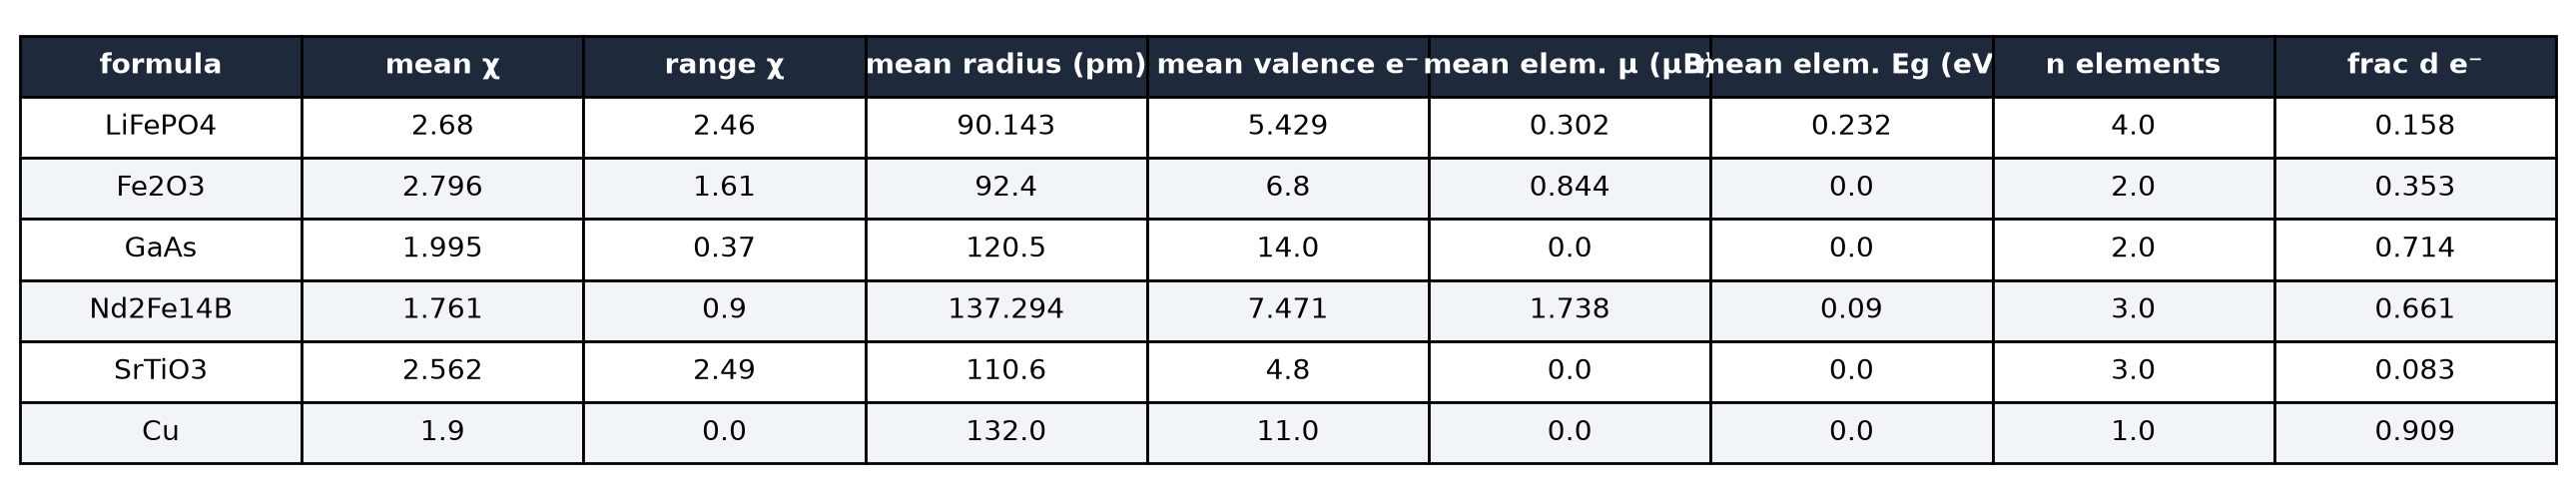
\includegraphics[width=\textwidth]{schematics/descriptor_examples.png}
  \caption{Extraction of physicochemical descriptors for example compositions.}
\end{figure}

\item \textbf{Exploring our Data:} before training, we analyzed every labeled dataset to
understand how the descriptors interact with each other and with the target variable. We
generated correlation heatmaps to identify strong associations between physicochemical
properties (such as electronegativity or valence-electron count) and the
stability/magnetism/metallicity labels. This step was crucial to verify that our engineered
features carry meaningful signals for classification. Figures~\ref{fig:corr}--\ref{fig:outliers}
show the Alexandria stability dataset (the largest one); the notebooks contain the same
analysis for every dataset.

\begin{figure}[H]
  \centering
  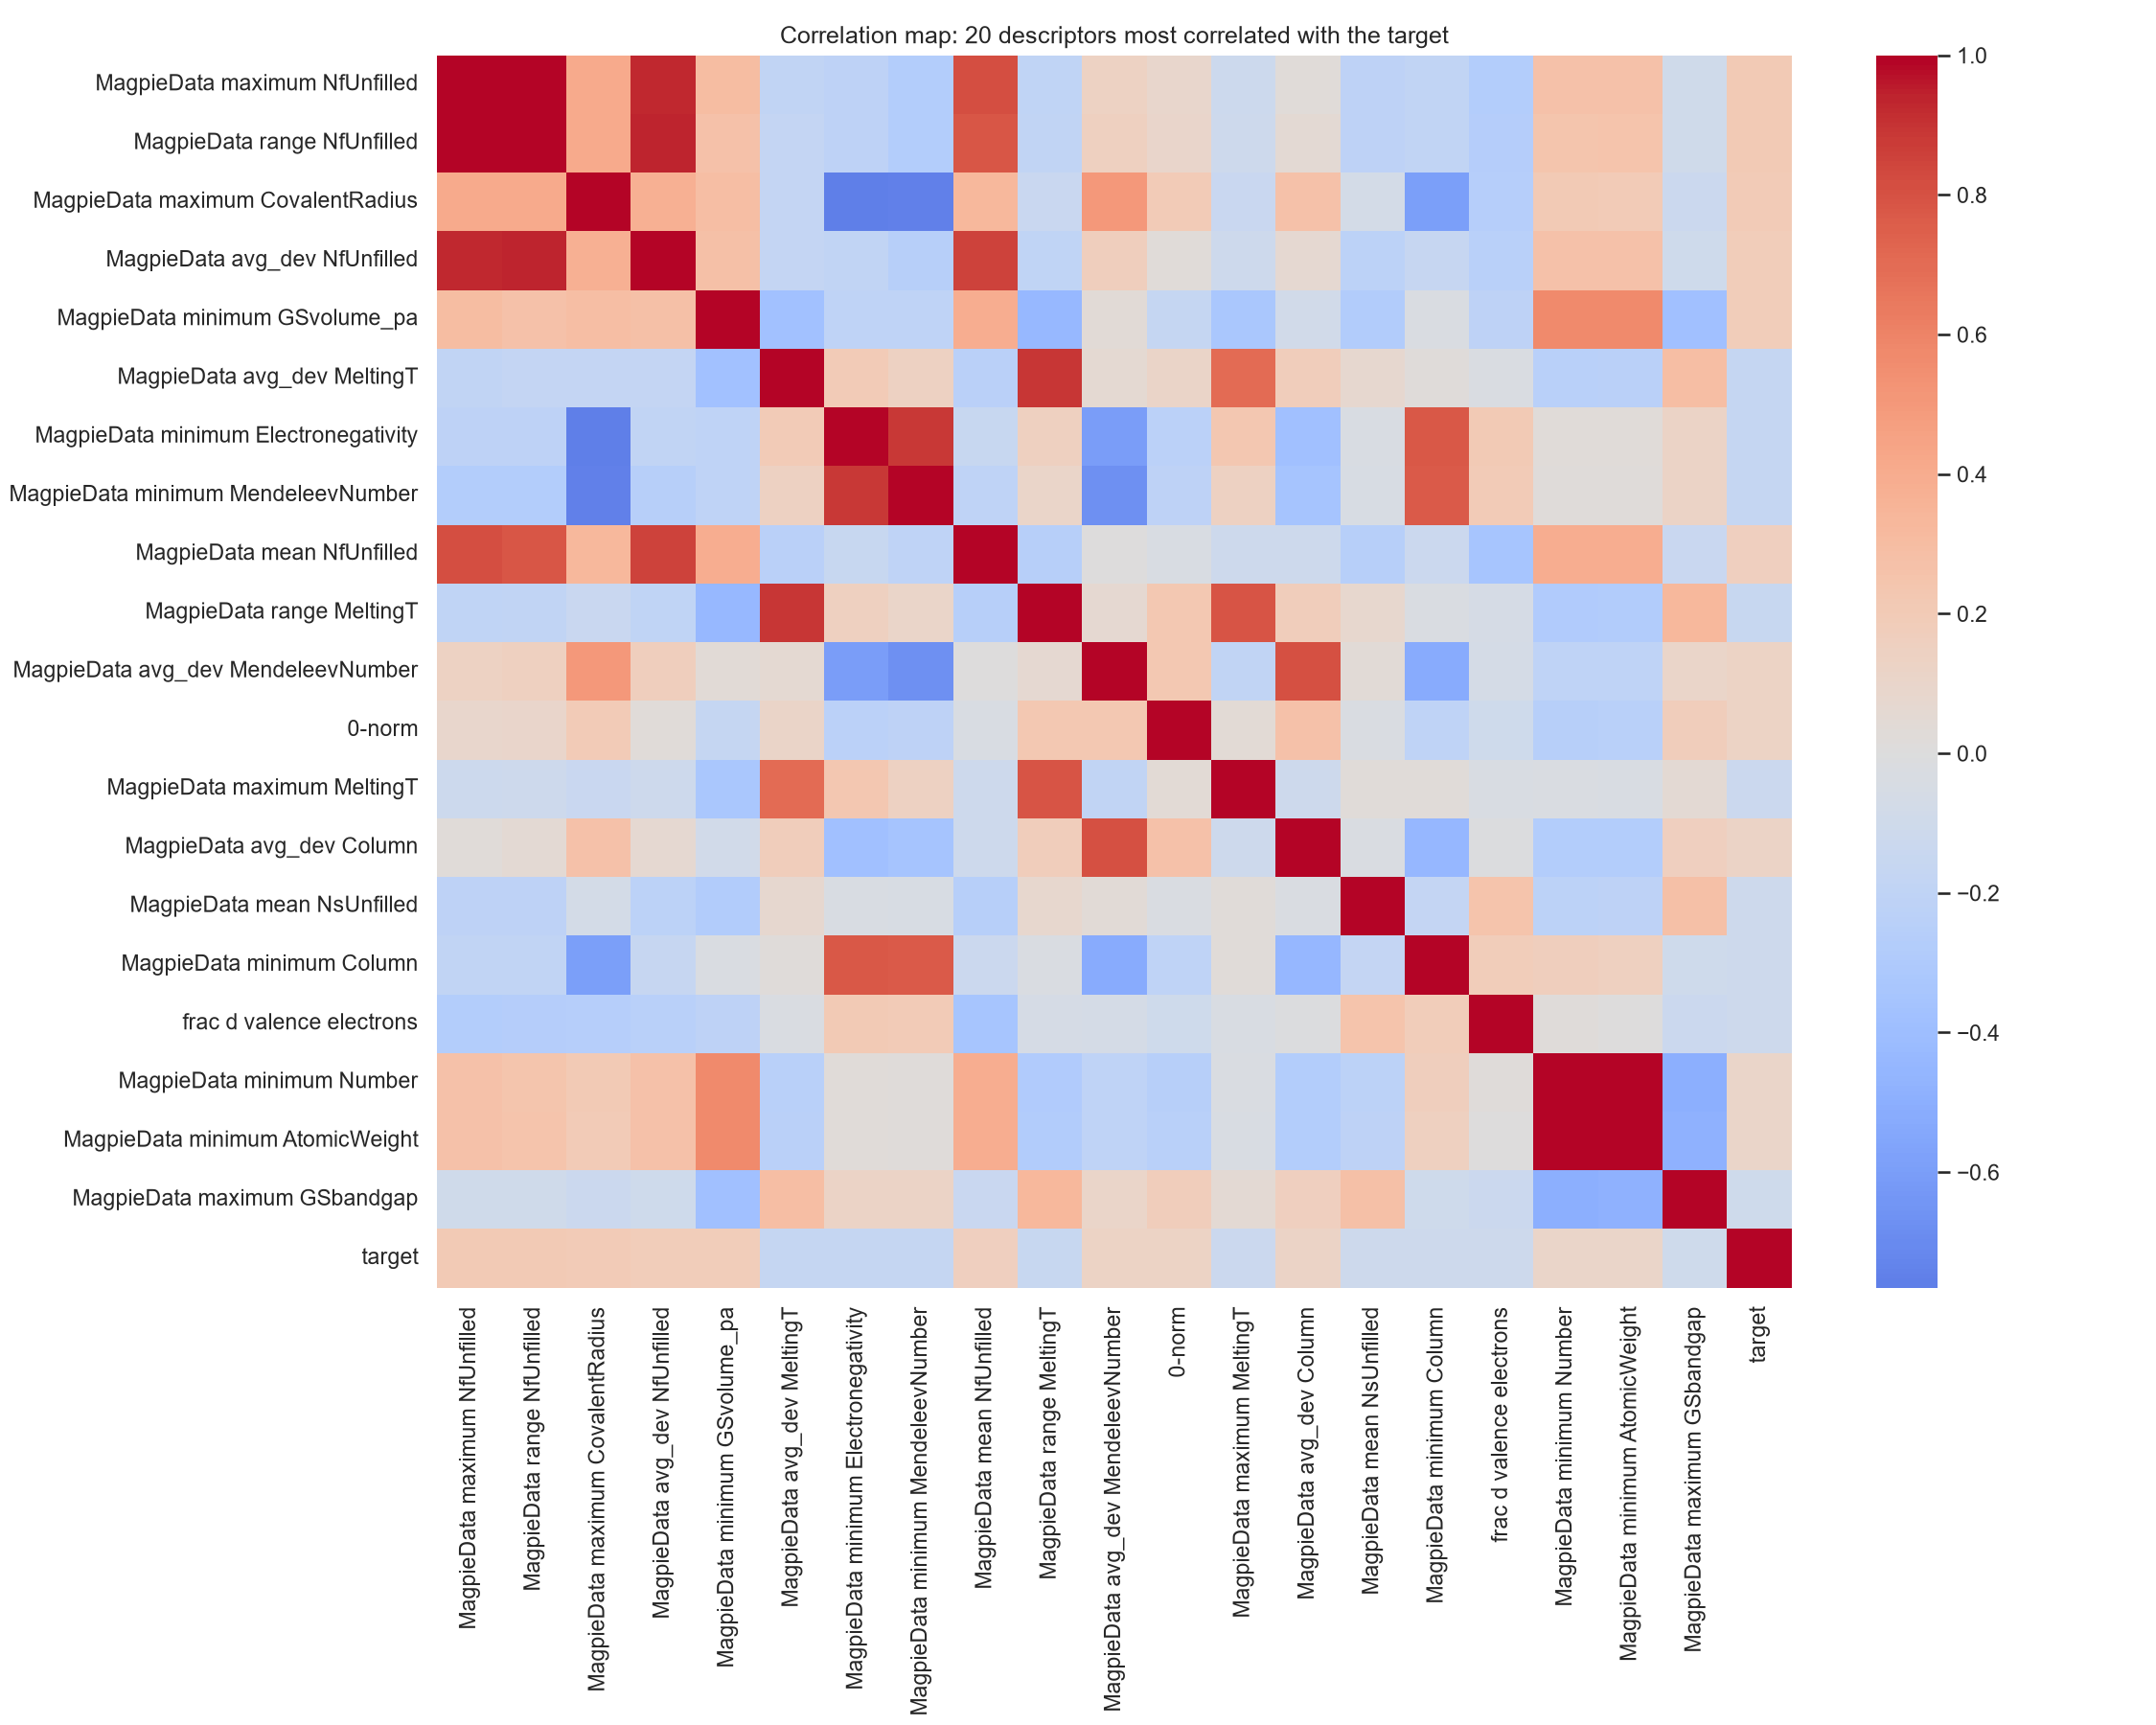
\includegraphics[width=0.82\textwidth]{stability/correlation_map.png}
  \caption{Correlation Map}\label{fig:corr}
\end{figure}

\begin{figure}[H]
  \centering
  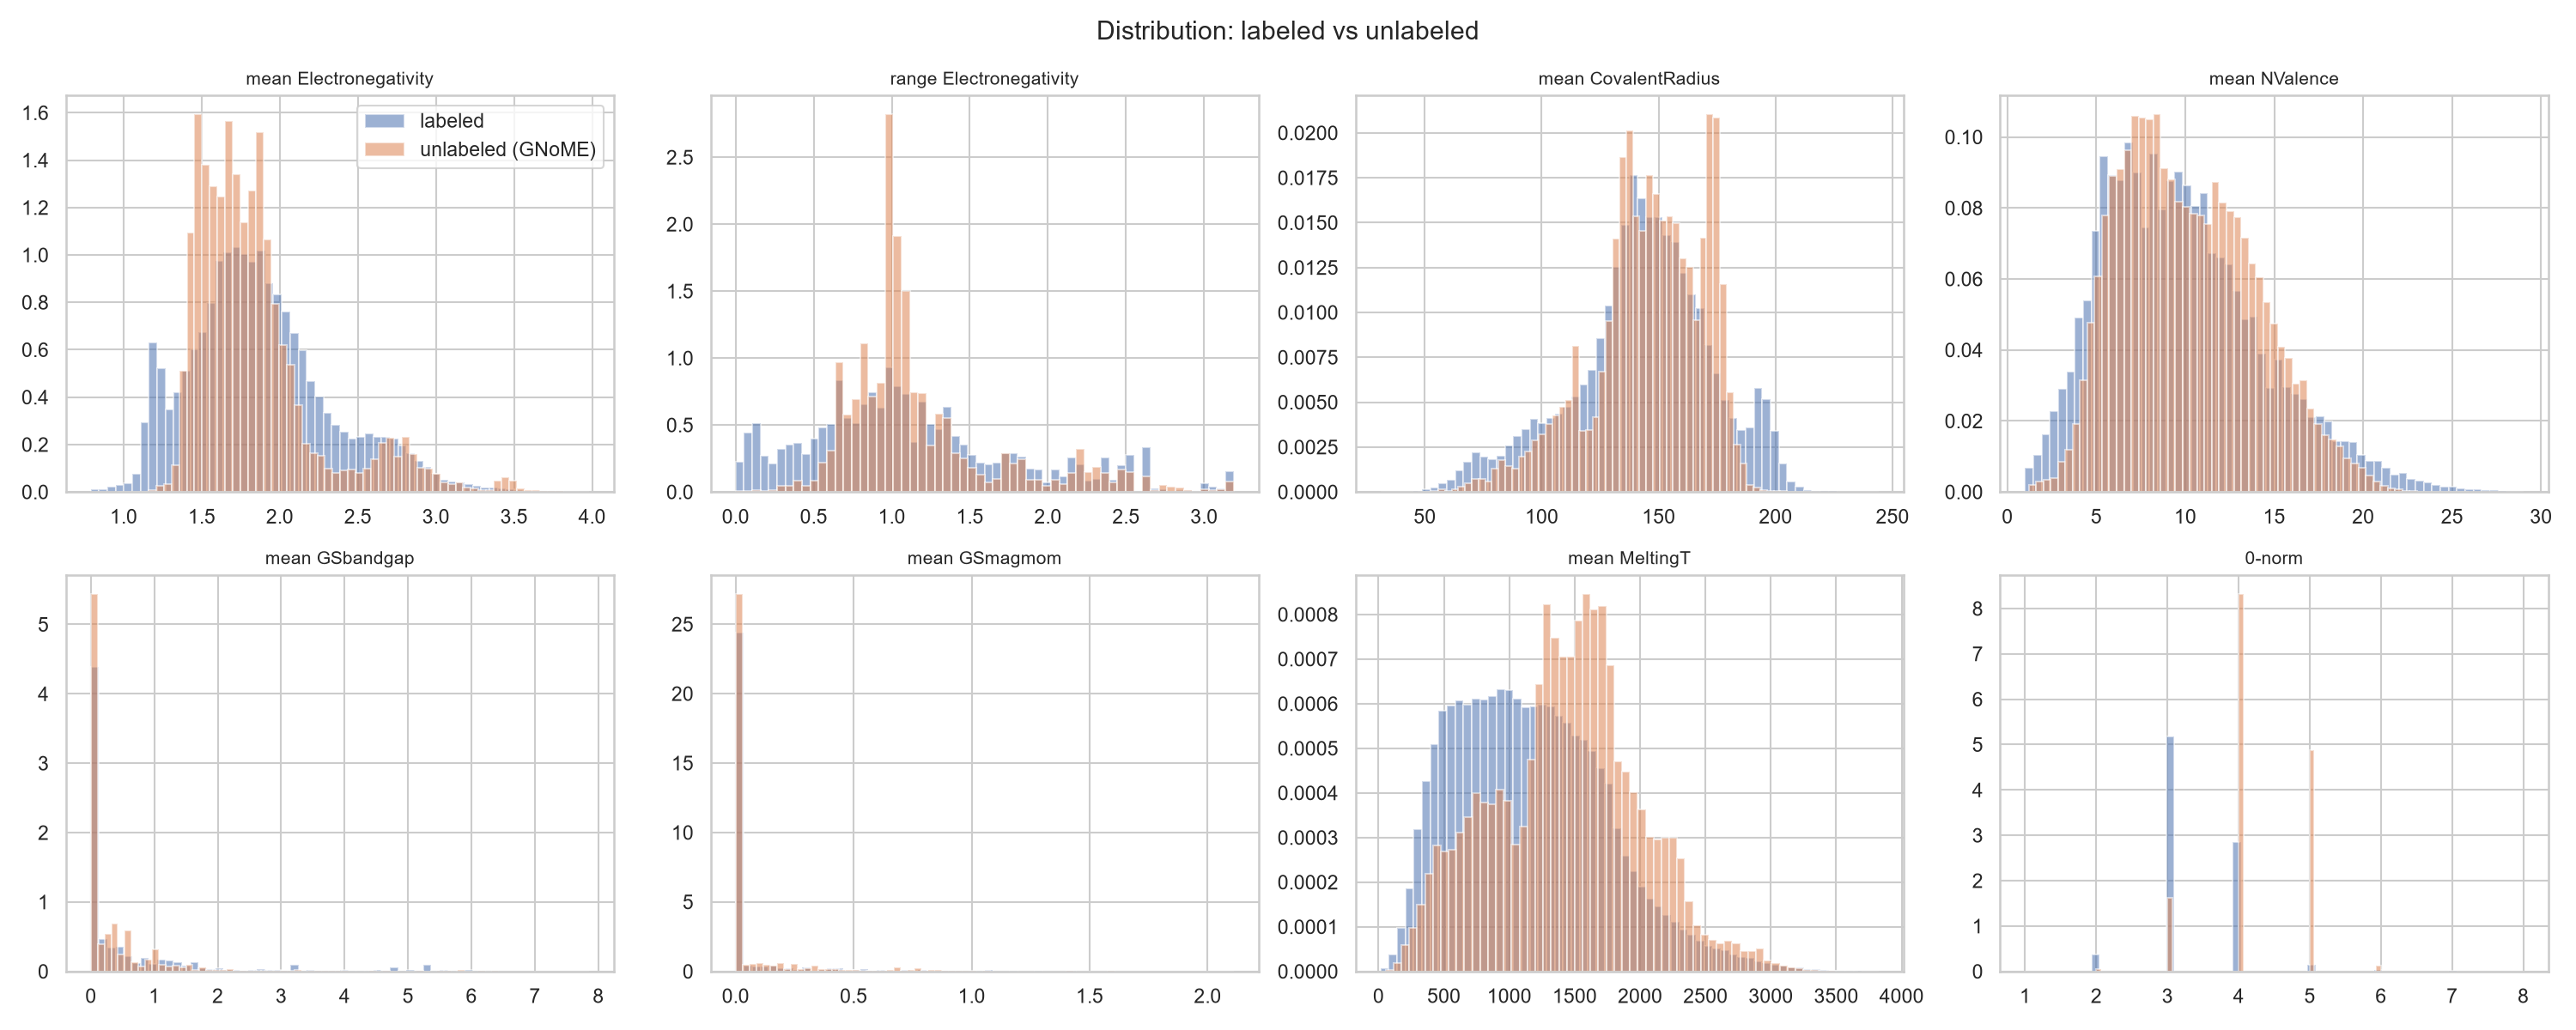
\includegraphics[width=\textwidth]{stability/labeled_vs_unlabeled.png}
  \caption{Distribution Labeled vs unlabeled}\label{fig:shift}
\end{figure}

The Kolmogorov--Smirnov tests confirm that labeled and unlabeled compositions are not drawn
from exactly the same distribution: for Alexandria most KS statistics stay below 0.25, whereas
for the Materials Project metallicity data they reach 0.43--0.48 (mean electronegativity,
melting temperature, number of elements). This distribution shift is an important factor in
the SSL results (Section~\ref{sec:discussion}).

\begin{figure}[H]
  \centering
  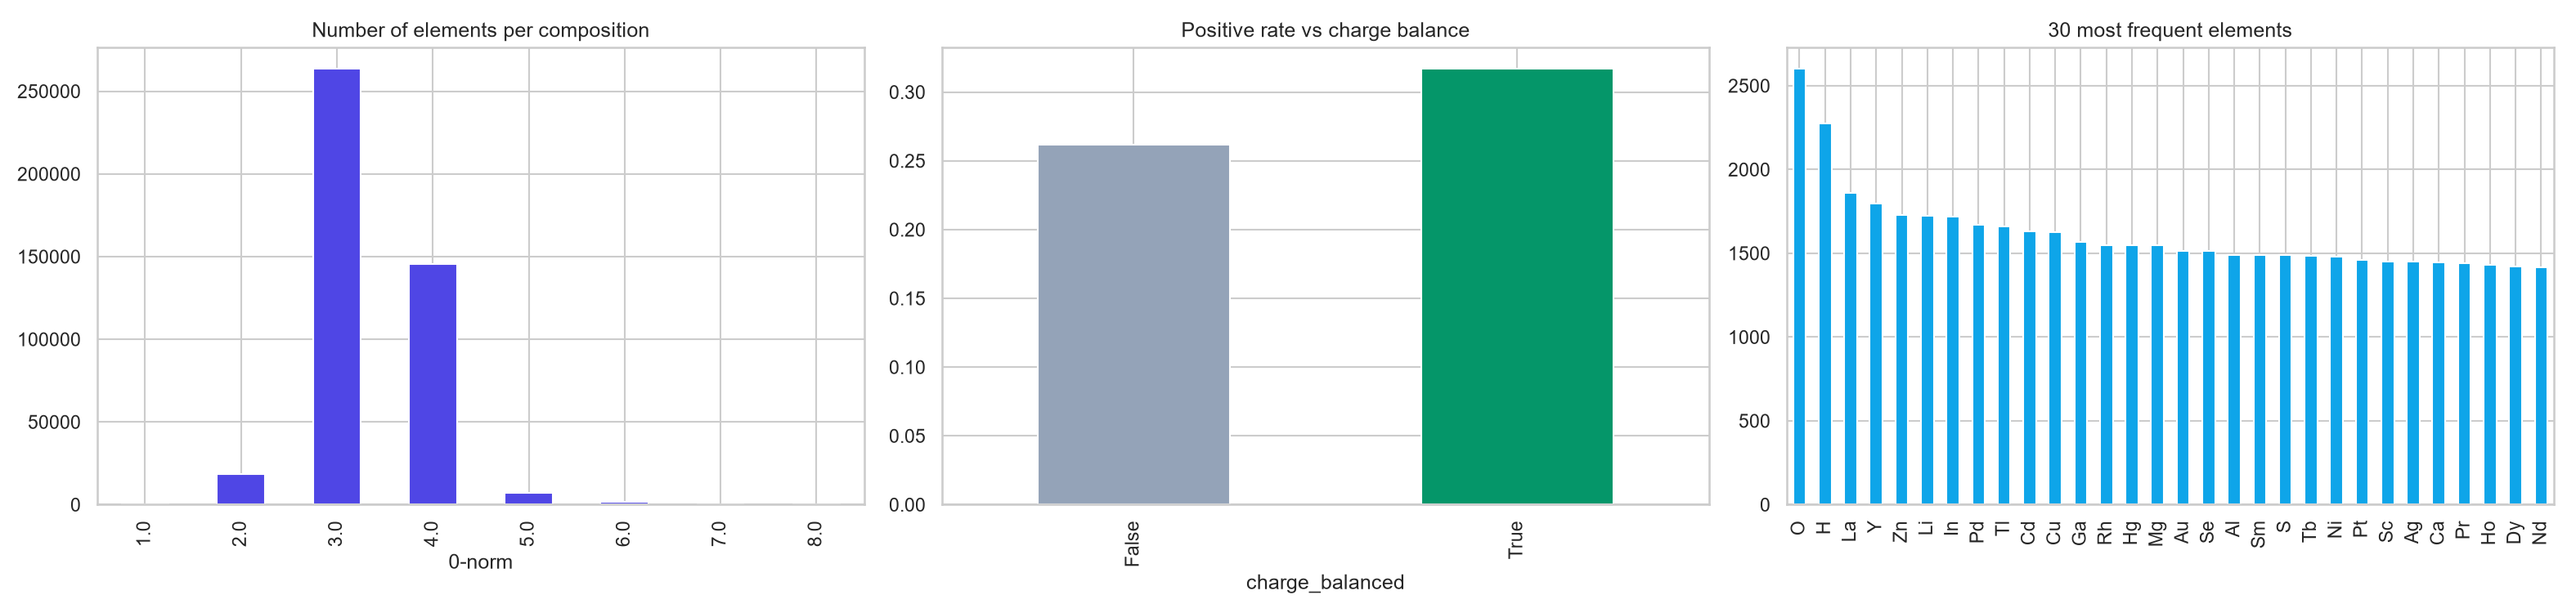
\includegraphics[width=\textwidth]{stability/chemical_rules.png}
  \caption{Chemical Rules}
\end{figure}

\begin{figure}[H]
  \centering
  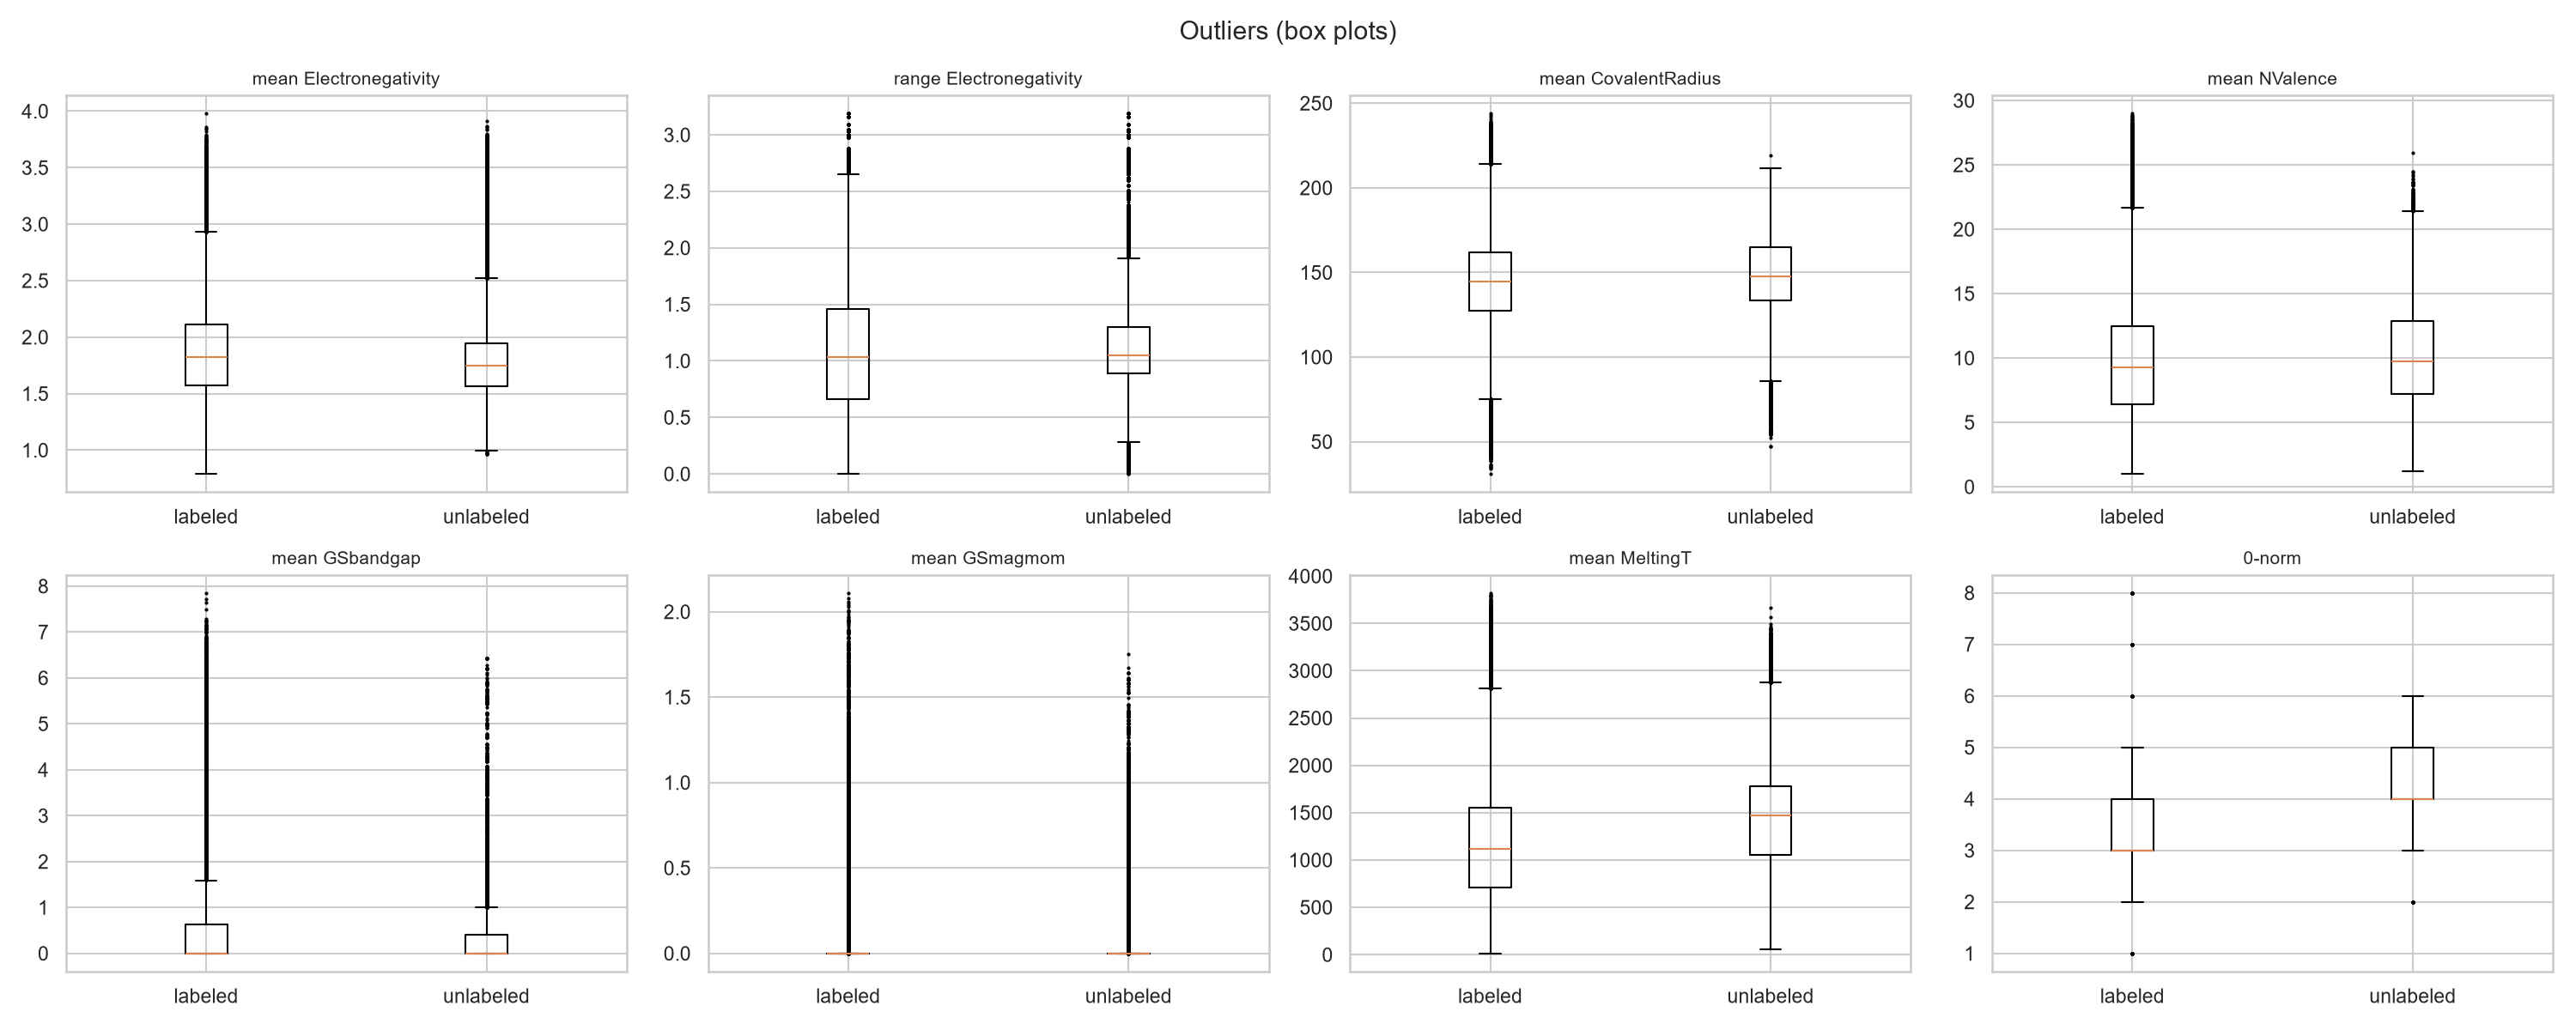
\includegraphics[width=\textwidth]{stability/outliers.png}
  \caption{Outliers}\label{fig:outliers}
\end{figure}

\item \textbf{Normalization and Scaling:} to ensure model stability, missing values are
imputed with the median, outliers are clipped at mean $\pm 3$ standard deviations (0.78\% of
the values for Alexandria, 0.95\% for Materials Project) and all features are standardized
with a \texttt{StandardScaler}. The preprocessing object is fitted on the training data only
and saved to ensure consistent transformation during inference.

\begin{figure}[H]
  \centering
  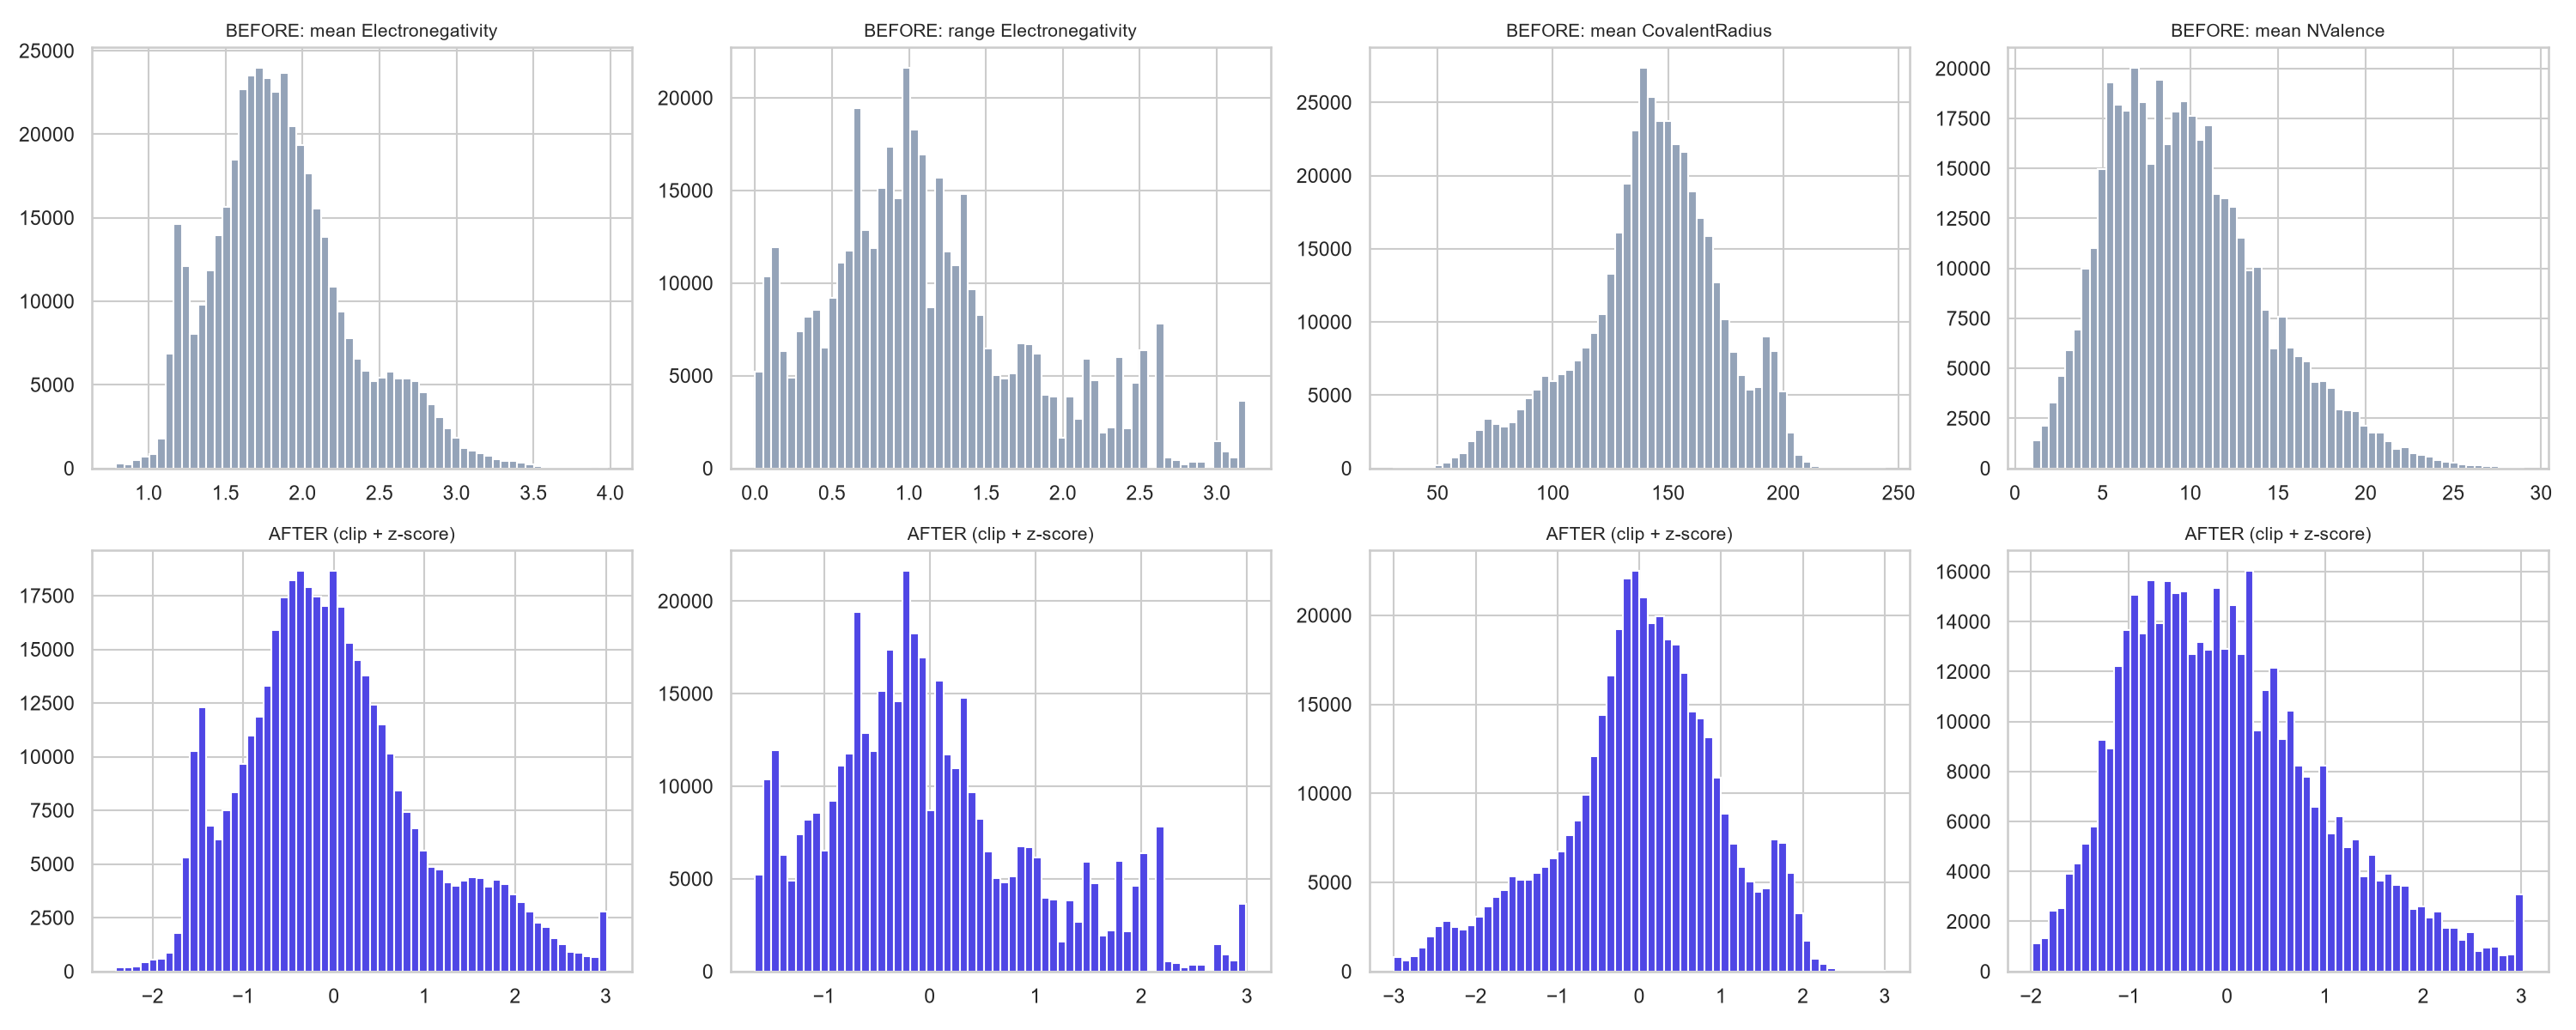
\includegraphics[width=\textwidth]{stability/normalization_before_after.png}
  \caption{Normalization of feature vectors (before and after clipping and z-scoring).}
\end{figure}

\item \textbf{Final Dataset Compilation:} the pipeline concludes by saving the processed
labeled and unlabeled datasets, ready for training. The output confirms the count of labeled
compositions, unlabeled compositions, and total features.

\begin{figure}[H]
\begin{console}
FINAL OUTPUT OF THE PREPROCESSING PIPELINE\\
==========================================================\\
metallicity : \MetalN{} labeled | 554,047 unlabeled (GNoME) | 142 descriptors | pos. rate \MetalPos{}\%\\
magnetism~~~: \MagN{} labeled | GNoME pool deduplicated | 142 descriptors | pos. rate \MagPos{}\%\\
stability~~~: \StabN{} labeled | 548,412 unlabeled (GNoME) | 142 descriptors | pos. rate \StabPos{}\%\\
band\_gap~~~~: \GapN{} labeled | 142 descriptors | pos. rate \GapPos{}\%\\
split: stratified 80/20 train/test, test set never used for training or tuning
\end{console}
\caption{Final output of the preprocessing pipeline showing dataset statistics.}
\end{figure}
\end{enumerate}
